\subsection{Data}
\subsubcomment{Written by Daniela Fichiu}

It is a truth universally acknowledged that a text analytics project's success must depend on the data set used. It is a truth that we would unfortunately firstly discover after having worked on the project for a while. 


Finding the perfect data set was an iterative process. It also began with a list: we composed a checklist of requirements that our data must meet. 
\begin{enumerate}
	\item A research paper must have an abstract and a set of associated keywords. 
	\item The abstract must not be riddled with spelling errors. 
	\item Each paper should have at least three keywords.
	\item The authors' names, the paper's title, and the link used to access the paper, the ref, should also be available.
\end{enumerate}

Every process iteration resembled a trial of some sorts, where the potential data candidate was the defendant. After multiple iterations, we settled for the Journal of Machine Learning Research, in short, Jmlr \cite{jmlr}, a peer-reviewed open access scientific journal covering only machine learning scientific papers.
On Jmlr \cite{jmlr}, research papers are organized into volumes. In the winter of 2020, when our project started, there were twenty available volumes, each one containing anywhere between fifty to two hundred fifty scientific papers. Each paper has three associated links: 
\begin{enumerate}
	\item The first link leads to a website where the paper's title, abstract, and the authors' names are listed. 
	\item The second link is used to access the paper in PDF format. 
	\item The third link, a BibTeX file, contains the paper's bibliography.
\end{enumerate}

We randomly sampled twenty papers: no abstract had spelling mistakes and each paper had at least four associated keywords. Jmlr \cite{jmlr}, seemed to be the perfect data source, as we had previously rejected Crossref \cite{crossref} because of the poor quality of the papers' abstracts.


The questions that had to be answered next were how to download the papers and where to store them. We concluded that Jmlr \cite{jmlr} must host anywhere between two thousand to four thousand papers. Saving them locally should not pose a problem. What Jmlr \cite{jmlr} did not offer was an API to download the papers. Manually downloading the papers was a task we were not ready to perform.The structured way the papers were saved on Jmlr \cite{jmlr}  gave rise to the idea of scraping the information we were interested in. 


Few things run smoothly from the beginning and require no further adjustments. A trial and error process riddled with subsequent tweaks is a rite of passage that transforms a theoretical great idea into a practical great idea.
\subsubsection{The First Attempt}
\subsubcomment{}
Randomly sampling the research papers showed that the first link was saved in one of two possible HTML elements, while the link with the PDF, the second link, appeared to be always saved in the same HTML element.


We used HTTP requests to access the two links and retrieve the PDF. From the first linked we extracted the paper's title, abstract, and the authors' names by parsing the page's HTML elements. Pdftotext \cite{p2t} and RegEx were used to extract the keywords from the HTTP response containing the paper's PDF. We saved the extracted information in a JSON file, creating a separate entry for each scraped paper.


The first problem we encountered was the inadequacy of the RegEx used to extract the keywords from the PDF: it did not work for every paper, as not all papers possessed the same structure. It would correctly extract the keywords from a set of papers, but then it would also extract other text. To solve this, we changed the expression to leave out the last keyword. Running the script took around an hour. 

\subsubsection{The Second Attempt} 
\subsubcomment{}
In the second trial, we only meant to address the problem of the "lost" keyword. Testing different RegEx expressions was a cumbersome task, as the script took one hour to run. To solve this, we switched from requests to Scrapy \cite{kouzis2016learning}, a web-crawling framework. We used Scrapy \cite{kouzis2016learning} to download the PDFs. The running time dropped from more than sixty minutes to one minute. 


The downside of using Scrapy \cite{kouzis2016learning} was the need for another pipeline to extract information. We were once again facing two problems. The first problem we had to confront was the missing ref, the link used to access the research papers. We had previously extracted the ref from an HTML element. We still had access to the refs, as Scrapy  \cite{kouzis2016learning}used them to download the PDFs, but nowhere to save them. The solution we found made use of the PDFs' names: we saved the PDFs under their ref. As the ref contained slashes, which were interpreted by Scrapy \cite{kouzis2016learning} as subdirectories, we changed them to semicolons using RegEx.


The second problem that needed to be addressed was how to efficiently extract information from the downloaded PDFs, also accounting for different structures. We decided to use GROBID \cite{GROBID}, a machine learning library for extracting information from PDFs into structured XML encoded documents with a particular focus on technical and scientific publications. We fed the downloaded PDFs into GROBID  \cite{GROBID} and parsed the resulting XMLs, saving the information in a JSON file. The final data set was generated using this approach.


\begin{figure}[h]
    \centering
    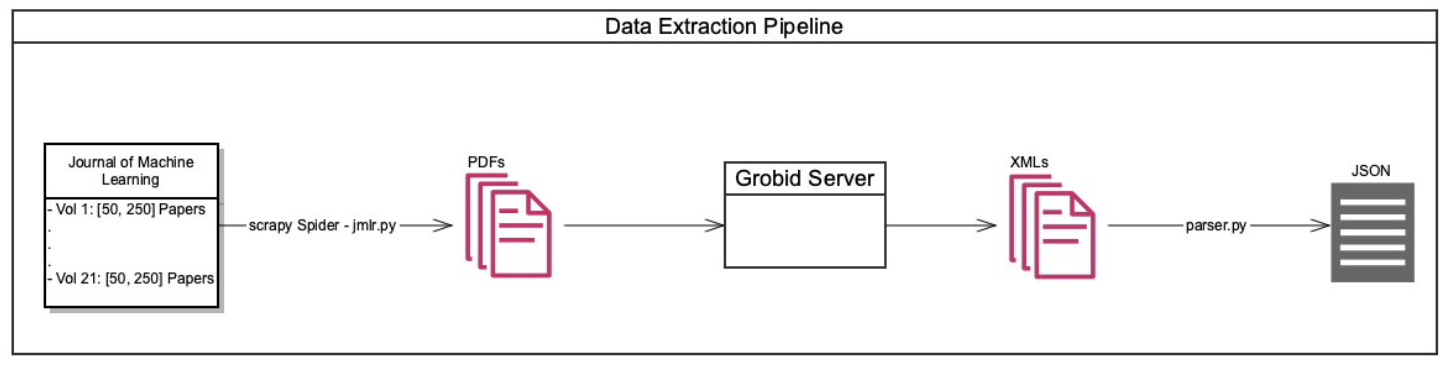
\includegraphics[width=1.0\linewidth]{imgs/data_pipeline.png}
    \caption{Complete pipeline from online paper source to extracted information in well-structured JSON file}
    \label{fig:data pipeline}
\end{figure}

\subsubsection{General Statistics}
\subsubcomment{}
Below we list some general statistics of our data set:
\begin{enumerate}
	\item The data set consists of 2230 research papers on the topic of mache learning.
	\item 20 papers posses no abstract.
	\item 159 papers have no keywords.
	\item The average number of keywords found in a research paper is 4.7
\end{enumerate}
